\documentclass[12pt]{article}
\parindent=0.25in

\setlength{\oddsidemargin}{0pt}
\setlength{\textwidth}{440pt}
\setlength{\topmargin}{0in}
\usepackage{amssymb}
\usepackage{amsfonts}
\usepackage{amsmath}
\usepackage{cancel}
\usepackage{latexsym}
\usepackage[center]{subfigure}
\usepackage{epsfig}
\usepackage{3952}
\usepackage{3952-thm}
\usepackage{pstricks,pst-node,pst-tree}
\usepackage{soul, xcolor}
\usepackage[backref, colorlinks,citecolor=blue,bookmarks=true]{hyperref}  


% \def\size{\mathop{\rm{size}}\nolimits}
% \def\depth{\mathop{\rm{depth}}\nolimits}
% \newtheorem{theorem}{Theorem}
% \newtheorem{lemma}{Lemma}
% \newtheorem{corollary}{Corollary}
% \newtheorem{fact}{Fact}
% \newtheorem{definition}{Definition}
% \newtheorem{claim}{Claim}
% \newenvironment{proof}{\noindent \textbf{Proof:}}{$\Box$}
% \newenvironment{proofsketch}{\noindent \textbf{Proof Sketch:}}
% \newcommand{\infint}{\int_{-\infty}^\infty}
% \newcommand{\intunit}{\int_{-1}^1}
% \newcommand{\binclass}{x \in \{0,1\}^n}
% \newcommand{\example}{\textbf{Example:} }
% \newcommand{\observation}{\textbf{Observation:} }
% \newcommand{\note}{\textbf{Note:} }
% \newcommand{\noisy}[1]{N_\epsilon(#1)}
% \newcommand{\noisens}[1]{ns_\epsilon(#1)}
% \newcommand{\eg}{{\it e.g.,\ }}
% \newcommand{\Inf}{{\mathrm{Inf}}}
% \newcommand{\PAR}{{\mathrm{PAR}}}
% \def\poly{\mathop{\rm{poly}}\nolimits}
% \def\eps{{\epsilon}}
% \newcommand{\E}{{\bf E}}
% \def\through{{,\ldots,}}


\pagestyle{headings}    % Go for customized headings

\newcommand{\handout}[5]{
   \noindent
   \begin{center}
   \framebox{
      \vbox{
    \parbox[t]{4in} {\bf #1 } \vspace{3mm}  {\hfill \bf #2 }
       \vspace{2mm}
       \hbox to 6.00in { {\Large \hfill #5  \hfill} }
       \vspace{1mm}
       \hbox to 6.00in { {\it #3 \hfill #4} }
      }
   }
   \end{center}
   \vspace*{1mm}
}

\hypersetup{linkcolor=magenta}

\begin{document}

\handout{MATH 3952 (Undergraduate Seminar): Quantum Information Theory}{Spring 2024}
{Organizer: Patrick Lei; Presenter: Liz Radway}
{Scribe: Mark Chen}{Lecture 1, Talk 1: January 29, 2024}

\thispagestyle{plain}
% \setcounter{section}{-1}
\section*{Chapter 0: Mathematical Background}
\begin{notation}
Bra-ket notation: such that $$
\langle u| v\rangle = \langle u||v\rangle
$$, where $\langle u|$ is conjugate transpose of $|u\rangle$. In this specific example, $\langle u|$ is called the ``bra" and $|v\rangle$ is called the ``ket". Particularly, $|u\rangle = \begin{bmatrix}
    u_1\\
    u_2\\
    \vdots\\
    u_n
\end{bmatrix}$ denotes a $n$-dimensional column vector. If not specified otherwise, we denote the space of ``bras" as $U$ and the space of ``kets" as $U^*$.
\end{notation}

\begin{definition}[Basis, and How it Works]
Suppose we are working with $U$ with a finite dimension, then what we mean is that it has a finite basis, say $n$-dimensional. Then, by Gram-Schmidt, orthonormal basis would always exist, and suppose the set of orthonormal basis of $U$ is $\{\Ket{e_1}, \Ket{e_2}, \ldots, \Ket{e_n}\}$. So, for some $v\in U$, we can write it as $$
v = \Sum{i}{1}{n}v_i\Ket{e_i}
$$. To make it more concise, we usually just write it as $$
\Ket{v} = \Sum{i}{1}{n}v_i\Ket{i}
$$
\end{definition}

\begin{definition}[Dual $\&$ Dual Basis]
From the above example of $\langle u|$ and $|u\rangle$, it is easy to appreciate the relationship between such pairs of elements. In fact, we denote $|u\rangle\in U$ and $\langle u|\in U^*$, and we call $U^*$ the dual space of $U$. In $U^*$, we have the dual basis $\{\Bra{e_1}, \Bra{e_2}, \ldots, \Bra{e_n}\}$.

Note that, to transition between $\Ket{v}$ and $\Bra{v}$, we have the following:
\begin{itemize}
    \item $\Ket{v} = \underset{i}{\sum}\Ket{i}\bk{i}{v}$.
    \item $\Bra{v} = \underset{i}{\sum}\bk{v}{i}\Bra{i}$.
\end{itemize}
\end{definition}

\begin{definition}[Dual $\&$ Dual Basis]
There is a bijection from $U$ to $U^*$, and we call it a dagger, denoted by ``$\dag$." Particularly, $\langle x| = \prt{|x\rangle}^\dag$ and $|x\rangle = \prt{\langle x|}^\dag$ (i.e. it goes both ways).
\end{definition}

\begin{proposition}
The following are basic properties of $\bk{u}{v}$ that handily follow from linear algebra.
\begin{itemize}
    \item $\bk{u}{v} = \bk{v}{u}^*$ (on a specific element, $(\cdot)^*$ denotes the conjugate transpose).
    \item Under linear combinations:
    \begin{itemize}
        \item $\prt{c_1\Ket{v_1}+c_2\Ket{v_2}}^\dag = c_1^* \Bra{v_1} + c_2^*\Bra{v_2}$.
        \item $\prt{c_1\Bra{v_1}+c_2\Bra{v_2}}^\dag = c_1^* \Ket{v_1} + c_2^*\Ket{v_2}$.
    \end{itemize}
\end{itemize}
\end{proposition}

\begin{definition}[Length / Norm, Orthogonal]
$||v|| = \sqrt{\bk{v}{v}}$. $u,v\in U$ are said to be orthogonal if $\bk{u}{v} = 0$.
\end{definition}

\begin{definition}[Probability Amplitude]\label{def:prob-amp}
$\bk{u}{v}$ describes the probability amplitude that a quantum system prepared in $\Ket{v}$ state will be found in $\Ket{u}$ state.
\end{definition}

\begin{definition}[Perfectly distinguishable]\label{def:perf-dist}
Recall definition \ref{def:prob-amp}, we see that if $\bk{u}{v} = 0$, then $u,v$ are perfectly distinguishable. In other words, if we prepare a quantum system in $\Ket{v}$ state, we will never find it in $\Ket{u}$ state.
\end{definition}

\begin{definition}[Operators]
In the context of this lecture, an operator is a linear endomorphism (i.e. a map from a space to itself). Notice that this definition of an operator is more restricted than the common sense, since usually when people say operators they probably mean neither linear nor an endomorphism.
\end{definition}

\begin{definition}[Adjoint or Hermitian Conjugate]
Hermitian conjugate of a linear map $A$, written as $A^\dag$, is defined by $$
\Bra{i}A^\dag\Ket{j} = \Bra{j}A\Ket{i}^*,\forall \Ket{i}, \Ket{j}\in \HHH
$$
\end{definition}

\begin{definition}[Normal, unitary, Hermitian]
An operator $A$ is said to be
\begin{itemize}
    \item \underline{Normal} if $A^\dag A = AA^\dag$.
    \item \underline{Unitary} if $A^\dag = A^{-1}$.
    \item \underline{Hermitian, or self-adjoint} if $A^\dag = A$.
\end{itemize}
Note that by the ways they are defined unitary and Hermitian operators both must be square matrices.
\end{definition}

\begin{definition}
A \underline{physically admissible} evolution of an isolated quantum system must be represented by a unitary operator.
\end{definition}

\begin{proposition}\label{prop:uni-map-preserve-ip}
Unitary maps preserve the inner product.
\end{proposition}
\begin{proof}
Write $\Ket{a'} = A\Ket{a}$ and $\Ket{b'} = A\Ket{b}$, then $\Bra{a'} = \Bra{a}A^\dag$. Then, $$
\bk{a'}{b'} = \Bra{a}A^\dag A\Ket{b} = \Bra{a}1\Ket{b} = \bk{a}{b}
$$
\end{proof}

\begin{fact}
An easy fact that follows from proposition \ref{prop:uni-map-preserve-ip} from definition is that norms are preserved under unitary maps, meaning that unit state vectors always get mapped to unit state vectors, which also means that unitary operators are the \hl{isometries of the Euclidean norm}.
\end{fact}

\section{Eigenvalues and Eigenvectors}
\begin{definition}[Operator]  Given an operator $A$, an eigenvector is a non-zero vector $\Ket{v}$ s.t. $$
    A\Ket{v} = \lambda \Ket{v}\text{ for some eigenvalue } \lambda \in \CC
$$
\end{definition}

\begin{definition}[Spectrum]
It may be obvious from the above equation that $$
A\Ket{v} = \lambda \Ket{v}\iff \det(A - \lambda I) = 0
$$, so the set of all such $\lambda$ is called the spectrum, denoted as $$
\sigma(A) = \{\lambda \in \C \mid \det(A-\lambda I) = 0\}
$$
\end{definition}

\begin{definition}[Eigenspace projector]
Firstly, define $$
\underset{i}{\sum}\lambda_i\Ket{v_i}\Bra{v_i}
$$, and we call each $P_i = \lambda_i\Ket{v_i}\Bra{v_i}$ an eigenspace projector, or an projector.

Let's inspect why this is important. A projector $P_i$ is one such that $P_i^\dag = P$ and $P^2 = P$.

Such a projector is derived from the following.
\begin{itemize}
    \item Normal operators have orthogonal eigenvectors. That is, $\bk{v}{u} = 0$ for $v\neq u$.
    \item Since eigenvectors can always be scaled, we can now just assume that these eigenvectors are just orthonormal.
    \item Thus, if we have the eigenpair $(\lambda_i, \Ket{v_i})$, we also have an orthornormal basis $\{\Ket{1}, \Ket{2}, \ldots, \Ket{n}\}$, which can be represented as an orthonormal.
    \item So, clearly, we can write (recall: $U = \underset{i}{\sum}\Ket{i}\Bra{v_i}$, and so $U^\dag = \underset{j}{\sum}\Ket{v_i}\Bra{j}$): $$
    \begin{aligned}
    UAU^\dag
        &= \underset{i,j}{\sum}\Ket{i}\Bra{v_i} A\Ket{v_j}\Bra{j}\\
        &= \underset{i,j}{\sum}\Ket{i}\Bra{v_j} \lambda_j \Ket{v_i}\Bra{j}\\
        &= \underset{i,j}{\sum}\lambda_j\Ket{i}(\bk{v_i}{v_j})\Bra{j}\\
        &= \boxed{\underset{i}{\sum}\lambda_i\Ket{i}\Bra{i}} \overset{\text{def}}{=} D\\
    \iff A
        &= U^\dag DU = \underset{i}{\sum}\lambda_i\Ket{v_i}\Bra{v_i}
    \end{aligned}
    $$. \hl{The RHS is called the spectral decomposition of $A$}.
\end{itemize}
\end{definition}

\begin{proposition}\label{prop:unity-of-projectors}
Projectors can only have eigenvalues of $0$ or $1$.
\end{proposition}
\begin{proof}
Notice that we have already stated that the projectors are required to be $P = P^\dag$ and $P^2 = P$. From $P^2 = P\implies P^2 - P = 0$. Thus, the eigenvalue, $\lambda$, for $P^2-P$ must satisfy $$
\begin{aligned}
(P^2 - P) \Ket{v} = (\lambda^2 - \lambda) \Ket{v}
    &= 0 \\
(\lambda^2 - \lambda)
    &= 0 \\
\lambda (\lambda - 1)
    &= 0
\end{aligned}
$$, which means that $\lambda = 0$ or $\lambda = 1$.
\end{proof}

\begin{proposition}\label{prop:basic-tr-eigenvalues} Basic facts why the spectrum / eigenvalues are useful:
\begin{itemize}
    \item $\Trace{A} = \underset{\lambda\in \sigma(A)}{\sum} \lambda$.
    \begin{proof}
        $$
        \begin{aligned}
            \Trace{A}
                &= \Trace{U^\dag D U} \\
                &= \Trace{D UU^\dag} \\
                &= \Trace{D} \\
                &= \underset{i}{\sum} \lambda_i
        \end{aligned}
        $$
    \end{proof}
    \item $\Det{A} = \underset{\lambda\in \sigma(A)}{\prod} \lambda$.
    \begin{proof}
        $$
        \begin{aligned}
            \Det{A}
                &= \Det{U^\dag D U} \\
                &= \Det{U^\dag}\Det{D}\Det{U} \\
                &= \Det{D}\Det{U^\dag}\Det{U} \\
                &= \Det{D}\Det{U^\dag U} = \Det{D}\cdot 1 \\
                &= \Det{D}\\
                &= \underset{i}{\prod} \lambda_i
        \end{aligned}
        $$
    \end{proof}
\end{itemize}
\end{proposition}

\begin{fact}\label{fact:function-on-spec}[Extending functions to linear maps]
The spectral decomposition of a normal operator gives an effective way of calculating the action of a function on a matrix. If $f: \C\rightarrow \C$ is a function, then we can define $$
f(A) = \underset{i}{\sum} f(\lambda_i) \Ket{v_i} \Bra{v_i}
$$
\end{fact}

\begin{example}
An example that connects proposition \ref{prop:unity-of-projectors}, \ref{fact:function-on-spec}, and the requirement that $P^2 = P$ is to consider $f(A) = A^2$: $$
\begin{aligned}
A^2
    &= \prt{\underset{i}{\sum}\lambda_i\Ket{v_i}\Bra{v_i}}\prt{\underset{i}{\sum}\lambda_i\Ket{v_i}\Bra{v_i}}\\
    &= \underset{i,j}{\sum}\lambda_i\lambda_j\Ket{v_i}\bk{v_i}{v_j}\Bra{v_j}\\
    &= \underset{i}{\sum}\lambda_i^2\Ket{v_i}\Bra{v_j}
\end{aligned}
$$. Notice how this totally works for $P^2 = P$, because proposition \ref{prop:unity-of-projectors} just showed that $\lambda_i=1$ or $0$, and $1^2 = 1, 0^2 = 0$, which means $\lambda_i^2 = \lambda_i$ regardless, so it is indeed the case that $$
P^2 = P
$$
\end{example}

\section{$\HHH$ Hilbert space to describe quantum states}
\begin{itemize}
    \item We want $\HHH$ to have $n$ dimensions, if our quantum system has $n$ perfectly distinguishable states (as defined in \ref{def:perf-dist}).
    \item Any $\Ket{v}\in \HHH$ is a valid quantum state if $\bk{v}{v} = 1$.
    \item Phase of the quantum state doesn't matter. For instance, $e^{i\gamma}\Ket{v}$ and $\Ket{v}$ describe the same state.
\end{itemize}

\section{Outer Product}
We call $\bk{u}{v}$ the inner product, then we can also have $\Ket{u}\Bra{v}$ as the outer product. Notice hat the two are fundamentally different, because the former is a single element (in $\CC$) while the latter is an $n\times n$ matrix (i.e. a linear transformation).

\begin{proposition}
$A = \kb{a}{b}$, $B = \kb{c}{d}$. Then, $$
BA = \Ket{c}\bk{d}{a}\Bra{b}
$$, but we already know that $\bk{d}{a}\in \CC$, so it is just a constant that is commutative with the other two vectors. So, $$
BA = \bk{d}{a}\kb{c}{b}
$$, which is just a constant times a single linear map.
\end{proposition}

\begin{proposition}\label{prop:can-be-expressed-as-outer-products}
Any operator on $\HHH$ can be expressed as a sum of outer products. Given an orthonormal basis $\{\Ket{e_i}\}_{i= 1, \ldots, n}$, any operator which maps the basis vectors $\Ket{e_i}$ to vectors $\Ket{f_i}$ can be written as $$
\underset{i}{\sum} \kb{f_i}{e_i}
$$
\end{proposition}
\begin{proof}
We must have the property that $\bk{e_i}{e_j} = 0$ if $i\neq j$. Now, say, we have any random input $C$. Then, $$
\begin{aligned}
C\prt{\underset{i}{\sum} \kb{f_i}{e_i}}
    &= \underset{i}{\sum} C\kb{f_i}{e_i}
\end{aligned}
$$ (because matrix multiplications respect distributive law). But, then, for each of these, $$C\kb{f_i}{e_i}$$ will be linearly independent from each other for different values of $i$, because $\Bra{e_i}$'s are linearly independent as basis elements. So, this would effectively be the same as $C$ being acted on by $f_i$ for its component in the $e_i$ direction.\\
\end{proof}

\begin{fact}\label{fact:orth-basis-map-is-unitary}
Furthermore, if $\{\Ket{f_i}\}$ is also an orthonormal basis, then $$
\underset{i}{\sum} \kb{f_i}{e_i}
$$ is just a map from one orthonormal basis to another, which would be a unitary map that preserves inner product.
\end{fact}

\begin{fact}[Completeness]
A particular example of fact \ref{fact:orth-basis-map-is-unitary} is when $\{\Ket{f_i}\} = \{\Ket{e_i}\}$, then $$
\underset{i}{\sum} \kb{e_i}{e_i} = 1
$$ would be the unitary mapping. This is true for any orthonormal basis, and it is known as the \hl{completeness property} in quantum theory.

This turns out to be very useful. Consider $$
\begin{aligned}
\Ket{v}
    &= 1\cdot \Ket{v}\\
    &= \underset{i}{\sum} \kb{e_i}{e_i}\Ket{v}\\
    &= \underset{i}{\sum} \Ket{e_i}\bk{e_i}{v}\\
    &= \underset{i}{\sum} v_i\Ket{e_i}
\end{aligned}
$$
\end{fact}

\begin{proposition}[Adjoint of outer product]
$\prt{\kb{a}{b}}^\dag = \kb{b}{a}$
\end{proposition}

\section{Trace}
\begin{definition}
As we have proved in proposition \ref{prop:basic-tr-eigenvalues}, $\Trace{A}$ is the sum of eigenvalues of $A$.
\end{definition}

\begin{definition}\label{defn:alt-tr-def}
Alternatively, $$
\Trace{A} = \underset{k}{\sum}\Bra{e_k}A \Ket{e_k} = \underset{k}{\sum}\bk{e_k}{f_k} \bk{e_k}{e_k} = \underset{k}{\sum}\bk{e_k}{f_k} = \underset{k}{\sum}A_{kk}
$$ (note that this is by citing proposition \ref{prop:can-be-expressed-as-outer-products} to break down $A$ into some sum of outer products of the form).
\end{definition}

\begin{proposition}\label{prop:alt-tr-def}
What is phrased in definition \ref{defn:alt-tr-def} directly leads to an alternative way of understanding $\Trace$ as: $$
\mathsf{Tr}: \kb{b}{a} \rightarrow \bk{a}{b}
$$; i.e. it turns outer products to inner products. This is why:$$
\begin{aligned}
\Trace{\kb{b}{a}}
    &= \underset{k}{\sum}\Bra{e_k}\kb{b}{a}\Ket{e_k}\text{, by directly applying definition \ref{defn:alt-tr-def}}\\
    &= \underset{k}{\sum}\underset{\in \CC}{\underbrace{\bk{e_k}{b}}}\underset{\in \CC}{\underbrace{\bk{a}{e_k}}}\\
    &= \underset{k}{\sum}\Bra{a}\underset{=1}{\underbrace{\prt{\kb{e_k}{e_k}}}}\Ket{b}\\
    &= \underset{k}{\sum}\bk{a}{b}\text{, no longer depends on $k$}\\
    &= \bk{a}{b}
\end{aligned}
$$
\end{proposition}

\begin{remark}
Notice that proposition \ref{prop:alt-tr-def} works against any basis, because it is introduced arbitrarily and cancelled out arbitrarily with itself, so any basis would work. That is, the trace doesn't depend on the choice of basis.
\end{remark}

\begin{proposition}
Traces have the following properties:
\begin{itemize}
    \item (Cyclic) $\Trace{ABC} = \Trace{CAB} = \Trace{BCA}$. Notice that this is not general commutativity (``permutation invariant"), but just the equality between the ``cyclic permutations".
    \item (Linearity) $\Trace{\alpha A + \beta B} = \alpha\Trace{A} + \beta \Trace{B}$, where $A,B$ are square matrices and $\alpha, \beta\in \CC$.
\end{itemize}
\end{proposition}

\section{Probability}
\begin{definition}
The probability can be described formally with a three-tuple $(\Omega, \FFF, P)$, where
\begin{itemize}
    \item $\Omega$ is the sample space (the set of all possible outcomes).
    \item $\FFF$ is the events space, which is the set of sets of outcomes. Specifically, we can describe some event as a set, like flipping two coins and get exactly one head corresponds to the event $\{HT, TH\}$.
    \item $P$ is the probability function which assigns to any event a probability of value in $[0,1]$. In other words, $\FFF$ is the set of subsets of $\Omega$.
\end{itemize}

This definition puts probability right up the alley of measure theory.
\end{definition}

\begin{definition}
Other crucial definitions:
\begin{itemize}
    \item (Mutually exclusive) $\Pr[A\cap B] = 0$.
    \item (Independent) $\Pr[A\cap B] = \Pr[A] \Pr[B]$.
\end{itemize}

Typically, when we say mutually exclusive, we mean a single run of an experiment. Independent, on the other hand, implies multiple runs.
\end{definition}

\begin{proposition}[PIE]
$\Pr[A\cup B] = \Pr[A] + \Pr[B] - \Pr[A\cap B]$
\end{proposition}

\begin{definition}[Conditional probability]\label{defn:cond-prob}
$\Pr[B\mid A] = \frac{\Pr[A\cap B]}{\Pr[A]}$
\end{definition}

\begin{corollary}
An easy corollary of definition \ref{defn:cond-prob} is that $$
\begin{aligned}
\Pr[B\mid A]
    &= \frac{\Pr[A\cap B]}{\Pr[A]}\\
    &= \frac{\Pr[A]\Pr[B]}{\Pr[A]}\\
    &= \Pr[B]
\end{aligned}
$$
\end{corollary}

\begin{theorem}[Bayes's Theorem]
Let $A,B$ be events such that $\Pr[B]\neq 0$, then $$
\begin{aligned}
\Pr[A\mid B]
    &= \frac{\Pr[A\cap B]}{\Pr[B]} = \frac{\Pr[A\cap B]}{\Pr[A]}\frac{\Pr[A]}{\Pr[B]}\\
    &= \Pr[B\mid A]\frac{\Pr[A]}{\Pr[B]} = \frac{\Pr[B\mid A]\Pr[A]}{\Pr[B]}
\end{aligned}
$$
\end{theorem}
\newpage

\setcounter{section}{0}
\section*{Chapter 1: Quantum Interference}
\section{Probability Amplitude}
\begin{definition}\label{defn:prob-amp}
Probability Amplitude is the fundamental blocks of quantum probability, which can be characterized by the following:
\begin{itemize}
    \item The probability amplitude $\alpha\in \CC$, meaning it can be both negative or imaginary.
    \item (\textbf{Born's Rule}, due to Max Born) $|\alpha|^2 = P\in [0,1]$.
    \item For $\alpha_1, \alpha_2\in \CC$ that are probability amplitudes:
    \begin{itemize}
        \item (if $\alpha_1, \alpha_2$ are sequence of events) $\alpha = \alpha_1\alpha_2$.
        \item (if $\alpha_1, \alpha_2$ are mutually exclusive) $\alpha = \alpha_1 + \alpha_2$.
    \end{itemize}
\end{itemize}
\end{definition}

\begin{example}[Why is definition \ref{defn:prob-amp} useful?]\label{eg:prob-amp}
Consider a physical system that can get from configuration state $A$ to state $B$, where there are two paths to do so, denoted $z_1, z_2$. In the classical model, it is simply $P = P_1 + P_2$. But, using the probability amplitude: we have $$
\begin{aligned}
P
    &= |\alpha|^2 = |\alpha_1 + \alpha_2|^2 \\
    &= (\alpha_1 + \alpha_2)(\alpha_1 + \alpha_2)^* = (\alpha_1 + \alpha_2)(\alpha_1^* + \alpha_2^*)\\
    &= \underset{|a_1|^2}{\underbrace{\alpha_1\alpha_1^*}} + \alpha_2\alpha_1^* + \alpha_1\alpha_2^* + \underset{|a_2|^2}{\underbrace{\alpha_2\alpha_2^*}}\\
    &= |a_1|^2 + |a_2|^2 + \alpha_2\alpha_1^* + \alpha_1\alpha_2^*
\end{aligned}
$$. Notice that, we can generally write $a_1 = |a_1|e^{i\gamma_1}$ and $a_2 = |a_2|e^{i\gamma_2}$ where $\gamma_1, \gamma_2$ are phases of the states, so we can further rewrite the following: $$
\begin{aligned}
P
    &= |a_1|^2 + |a_2|^2 + |a_2|e^{i\gamma_2}|a_1|e^{-i\gamma_1} + |a_1|e^{i\gamma_1}|a_2|e^{-i\gamma_2} \\
    &= |a_1|^2 + |a_2|^2 + |a_1||a_2|\prt{e^{-i(\gamma_1-\gamma_2)} + e^{i(\gamma_1-\gamma_2)}} \\
\end{aligned}
$$. Finally, use Euler's identity, we realize that, since the two exponents are only different by their signs, the $\sin$ term cancels out under addition, and the $\cos$ term becomes $2x$'ed: $$
\begin{aligned}
P
    &= |a_1|^2 + |a_2|^2 + |a_1||a_2|\prt{e^{-i(\gamma_1-\gamma_2)} + e^{i(\gamma_1-\gamma_2)}} \\
    &= |a_1|^2 + |a_2|^2 + 2|a_1||a_2|\cos(\gamma_1-\gamma_2) \\
    &= P_1 + P_2 + 2\sqrt{P_1P_2}\cos(\gamma_1-\gamma_2)
\end{aligned}
$$. Clearly,
\begin{itemize}
    \item the $P_1 + P_2$ terms agree with the classic Kolmogorov model.
    \item $2|a_1||a_2|\cos(\gamma_1-\gamma_2)$ is called the \textbf{interference term}, which is the key difference from the classic model. Colloquially, this is saying that the actual physical system has a way to correlate the two seemingly mutually exclusive paths, by their phases.

    In addition, $\cos(\gamma_1-\gamma_2)$ can be positive or negative, meaning that it could both increase and decrease the total probability of getting from state $A$ to state $B$, depending on what $\phi_1, \phi_2$ are.  
\end{itemize}
\end{example}

\section{Modern Probability Theory Due to Kolmogorov}
\begin{definition}\label{defn:kol-prob}
The three axioms of the Kolmogorov modern probability theory:
\begin{enumerate}
    \item Once you identify all elementary outcomes or events, you can assign probabilities to them.
    \item The probabilities assigned must be in $[0,1]$, and a event that is certain to happen has a probability of $1$.
    \item (Additive axiom) Whenever an event can occur in several mutually exclusive ways, the probability for that event is the sum of probabilities for each way considered separately.
\end{enumerate}
\end{definition}

\begin{observation}[Counter-example]
The double-slit experiment is a counter-example to definition \ref{defn:kol-prob}: we would expect the particle to either pass through one slit or the other, so the result on the screen afterwards should just be two lines. But, experimentally, the result is something like:
\begin{center}
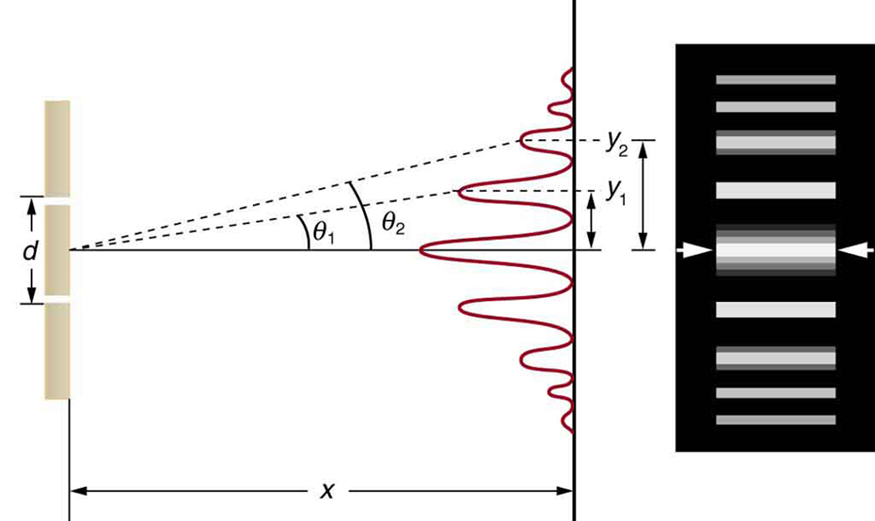
\includegraphics[width = 25em]{images/1.jpg}
\end{center}
That is, somehow, the photon acts like a wave, and splits into two as they each passes through the two slits, respectively, and then interfere with itself to achieve the final interference pattern.

This outcome of the double-slit experiment can be explained by the new probability model based on the probability amplitude described in definition \ref{defn:prob-amp}. That is, the interference term that is characterized by $\phi_1 - \phi_2$ is what characterizes the final distribution probability. As part of $\cos(\phi_1 - \phi_2)$, there are certain ways that it can be \textbf{destructive interference}, when $\cos(\phi_1 - \phi_2)$ is negative; or \textbf{constructive interference}, when $\cos(\phi_1 - \phi)$ is positive. So, really, the problem with the classical additive axiom that Kolmogorov proposed is that it needs to assume that the two paths through the two slits are mutually exclusive, but in the actual sense, they both happened simultaneously.

In a sense, what the quantum computer does is to explore all computational paths simultaneously, in some tangible way, and produce a probabilistic result based on all these alternative calculations.
\end{observation}

\section{Superposition}
Other than the two basis states $\Ket{\uparrow}$ and $\Ket{\downarrow}$, there are infinitely many other states as a superposition of these two basis states. One way to think about this is the spherical illustration of where a unit vector can be, with $\Ket{\uparrow}$ pointing up and equivalent to $\Ket{0}$ and $\Ket{\downarrow}$ pointing down and equivalent to $\Ket{1}$:
\begin{center}
    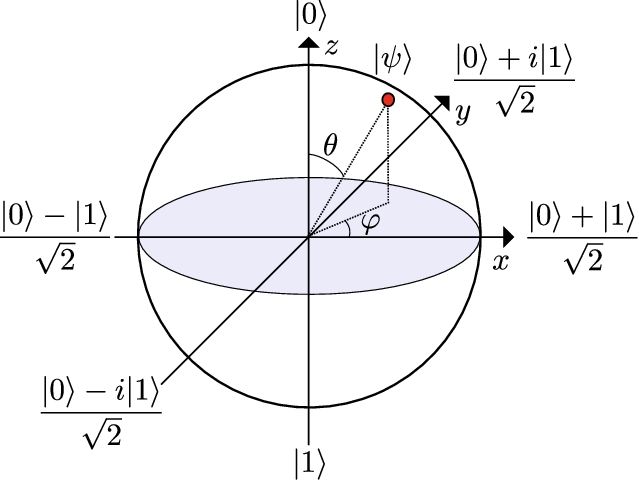
\includegraphics[width = 20em]{images/2.jpg}
\end{center}
(this image should give sufficient basics for how this sphere helps you think, and what kind of superpositions are allowed).

\section{Interferometers}
\begin{definition}[Interference experiments]
Interference experiments are a class of experiments, for which modern ones are conducted using internal degrees of freedoms of atoms and ions.

One example is the \textbf{Ramsey interferometry}, which is a generic name for an interference experiment where atoms are sent through two separate ``resonant interaction" zones known as the \textbf{\underline{Ramsey zones}}, separated by an intermediate ``\textbf{\underline{dispersive}} \textbf{\underline{interaction}}" zone.
\end{definition}

\subsection{A canonical example}
This example is a slight modification / generalization based on the actual experiment conducted by Serge Harcoche. In the following image, $\Ket{0} = \Ket{e}$ and $\Ket{1} = \Ket{g}$:
\begin{center}
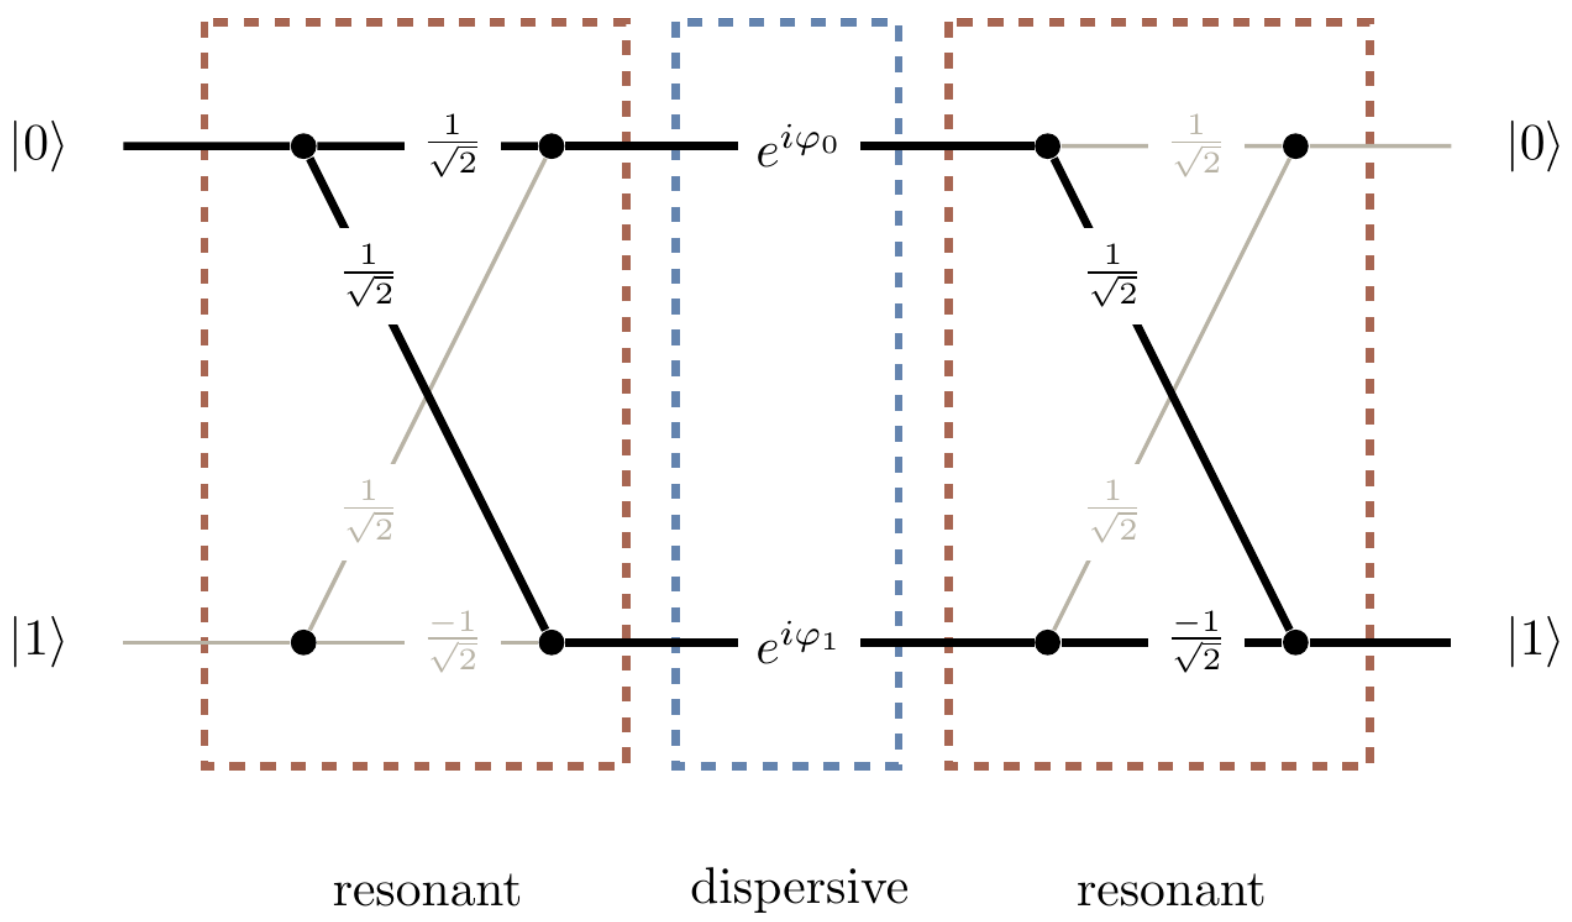
\includegraphics[width = 25em]{images/3.jpg}
\end{center}

\begin{definition}[Resonant $\&$ dispersive interaction zones]
The two terms are defined by how the field in each cavity interacts with the atom.
\begin{itemize}
    \item (Resonant interactions) Cavity field frequencies to match that of the atoms, so that the atom exchange energy with the cavity, going back and forth between $\Ket{1}$ and $\Ket{0}$.
    \item (Dispersive interactions) The field too off-resonance for the atom to exchange energy with it, but the field is nonetheless ``felt" which causes the phase of the atoms traveling through it to change.
\end{itemize}

$*$ The above diagram depicts a series of well-timed resonant-dispersive-resonant interactions.
\end{definition}

\begin{definition}[Direct computation of a specific probability amplitude]
We can prepare the initial internal state of the atom in either $\Ket{0}$ (excited) or $\Ket{1}$ (ground), but for the purpose of a specific example, we say that we start with $\Ket{0}$ and eventually observe a $\Ket{1}$. Then, its final state is the superposition of two possible paths traced out by the darker lines in the image: $$
\begin{aligned}
U_{10}
    &= \frac{1}{\sqrt{2}}e^{i\varphi_0}\frac{1}{\sqrt{2}} + \frac{1}{\sqrt{2}}e^{i\varphi_1}\frac{-1}{\sqrt{2}} = \boxed{\frac{1}{2}\prt{e^{i\varphi_0} - e^{i\varphi_1}}}\\
    &= \frac{1}{2}e^{i\frac{\varphi_0 + \varphi_1}{2}}\prt{e^{i\frac{\varphi_0 - \varphi_1}{2}} - e^{-i\frac{\varphi_0 - \varphi_1}{2}}} = \frac{1}{2}e^{i\frac{\varphi_0 + \varphi_1}{2}}\prt{2i\sin{\frac{\varphi_0-\varphi_1}{2}}} = \boxed{ie^{i\frac{\varphi_0 + \varphi_1}{2}}\sin{\frac{\varphi_0-\varphi_1}{2}}}
\end{aligned}
$$, by directly multiplying out the probability on each path since they are a sequence of events ($U_{10}$ denotes the probability that state $\Ket{1}$ is observed when the atom was initially in state $\Ket{0}$.)
\end{definition}

\begin{definition}[Direct computation of a specific probability]
With $U_{10}$ from above, we get its corresponding probability, $P_{10}$, quite simply: $$
\begin{aligned}
P_{10} = \left|U_{10}\right|^2
    &= \left|ie^{i\frac{\varphi_0 + \varphi_1}{2}}\sin{\frac{\varphi_0-\varphi_1}{2}}\right|^2\\
    &= \left|e^{i\frac{\varphi_0 + \varphi_1}{2}}\right|^2\left|i\sin{\frac{\varphi_0-\varphi_1}{2}}\right|^2 = 1\cdot \left|i \sin{\frac{\varphi_0-\varphi_1}{2}}\right|^2\\
    &= \prt{i \sin{\frac{\varphi_0-\varphi_1}{2}}}\prt{-i \sin{\frac{\varphi_0-\varphi_1}{2}}}\\
    &= \sin^2{\frac{\varphi_0 - \varphi_1}{2}}
\end{aligned}
$$ Recall that $$
\cos(2\theta) = \cos^2(\theta) - \sin^2(\theta) = \prt{\cos^2(\theta) + \sin^2(\theta)} - 2\sin^2(\theta) = 1-2\sin^2{\theta}
$$, where we let $\theta = \frac{\varphi_0 - \varphi_1}{2}$, which gives us: $$
P_{10} = \left|U_{10}\right|^2
    &= \sin^2{\theta} = \frac{1}{2}\prt{1 - \cos(2\theta)} = \boxed{\frac{1}{2}\prt{1 - \cos(\varphi_0 - \varphi_1)}}\\
$$ (this should remind us again of the difference between Kolmogorov and quantum probability: the first $\frac{1}{2}$ denotes the typical expected probability of one of the two equally likely options, while $-\frac{1}{2}\cos(\varphi_0 - \varphi_1)$ gives the interference adjustment).
\end{definition}

\begin{definition}[The one ring to rule it all: use matrix multiplication to tackle all possible paths in evolving quantum systems]
Again, inspect the system in the image pictured at the very beginning of 4.1 (current subsection). We can describe this whole system by the following matrix multiplication: $$
\begin{aligned}
\boxed{U}
    &= \frac{1}{\sqrt{2}}\begin{bmatrix}
        1 & 1\\
        1 & -1
        \end{bmatrix}\begin{bmatrix}
        e^{i\varphi_0} & 0\\
        0 & e^{i\varphi_1} 
        \end{bmatrix}\frac{1}{\sqrt{2}}\begin{bmatrix}
        1 & 1\\
        1 & -1
    \end{bmatrix}\\
    &= \frac{1}{2}\begin{bmatrix}
        e^{i\varphi_0} + e^{i\varphi_1} & e^{i\varphi_0} - e^{i\varphi_1}\\
        e^{i\varphi_0} - e^{i\varphi_1} & e^{i\varphi_0} + e^{i\varphi_1}
    \end{bmatrix} = \frac{1}{2}e^{i\frac{\varphi_0+\varphi_1}{2}}\begin{bmatrix}
        e^{i\frac{\varphi_0-\varphi_1}{2}} + e^{-i\frac{\varphi_0-\varphi_1}{2}} & e^{i\frac{\varphi_0-\varphi_1}{2}} - e^{-i\frac{\varphi_0-\varphi_1}{2}}\\
        e^{i\frac{\varphi_0-\varphi_1}{2}} - e^{-i\frac{\varphi_0-\varphi_1}{2}} & e^{i\frac{\varphi_0-\varphi_1}{2}} + e^{-i\frac{\varphi_0-\varphi_1}{2}}
    \end{bmatrix}\\
    &= \frac{1}{2}e^{i\frac{\varphi_0+\varphi_1}{2}}\begin{bmatrix}
        2\cos\frac{\varphi_0 - \varphi_1}{2} & 2i\sin\frac{\varphi_0 - \varphi_1}{2}\\
        2i\sin\frac{\varphi_0 - \varphi_1}{2} & 2\cos\frac{\varphi_0 - \varphi_1}{2}
    \end{bmatrix} = \boxed{e^{i\frac{\varphi_0+\varphi_1}{2}}\begin{bmatrix}
        \cos\frac{\varphi_0 - \varphi_1}{2} & i\sin\frac{\varphi_0 - \varphi_1}{2}\\
        i\sin\frac{\varphi_0 - \varphi_1}{2} & \cos\frac{\varphi_0 - \varphi_1}{2}
    \end{bmatrix} = \begin{bmatrix}
        U_{00} & U_{01}\\
        U_{10} & U_{11}
    \end{bmatrix}}
\end{aligned}
$$ (it is a good idea to work backward and see how the multiplication of the three matrices corresponds exactly to each path).
\end{definition}

\begin{proposition}[Dropping \textbf{global} phase factor]
It is customary to just write: $$
U
    = \begin{bmatrix}
        U_{00} & U_{01}\\
        U_{10} & U_{11}
    \end{bmatrix}
    = e^{i\frac{\varphi_0+\varphi_1}{2}}\begin{bmatrix}
        \cos\frac{\varphi_0 - \varphi_1}{2} & i\sin\frac{\varphi_0 - \varphi_1}{2}\\
        i\sin\frac{\varphi_0 - \varphi_1}{2} & \cos\frac{\varphi_0 - \varphi_1}{2}
    \end{bmatrix} = \boxed{\begin{bmatrix}
        \cos\frac{\varphi_0 - \varphi_1}{2} & i\sin\frac{\varphi_0 - \varphi_1}{2}\\
        i\sin\frac{\varphi_0 - \varphi_1}{2} & \cos\frac{\varphi_0 - \varphi_1}{2}
    \end{bmatrix}}
$$. We call $e^{i\frac{\varphi_0+\varphi_1}{2}}$ the global phase factor, which we have dropped in this case, at least partially because, for the purpose of defining probability amplitude here, $$
\left|e^{i\frac{\varphi_0+\varphi_1}{2}}\right| = 1
$$, which means it won't affect the eventual probability.
\end{proposition}

\end{document}
